\section{Project Structure}
The developed software is divided into three main components: the robot behavior implementation, a custom lightweight 2D simulator, and a Gazebo-based 3D simulation environment. \Cref{fig:software-structure} shows the dependency structure of the \texttt{botbrain} behavior library and the two simulates which will be further explained in the following sections.

\begin{figure}[H]
    \begin{center}
        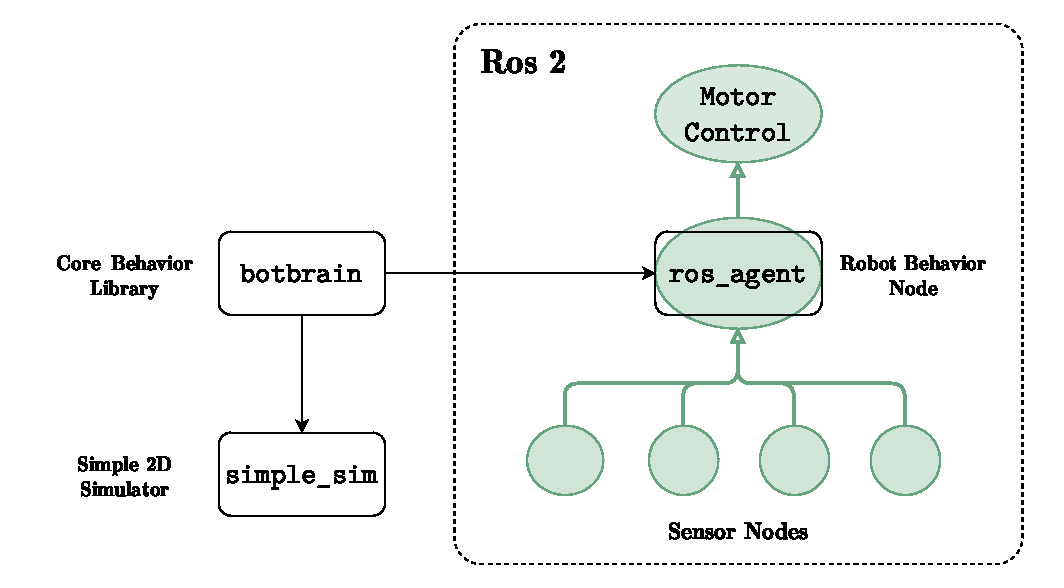
\includegraphics[width=0.95\textwidth]{figures/software-structure.pdf}
    \end{center}
    \caption{Software structure of the project. Black arrows indicate library dependencies, while green arrows denote ROS 2 communication through topics. Square boxes represent Rust crates and green circles represent ROS 2 nodes. The core library \texttt{botbrain} is ROS 2-independent and can be reused by the simple simulator without any dependency on ROS 2.}
    \label{fig:software-structure}
\end{figure}

\subsection{Simulated Hardware}
A simulated differential-drive robot equipped with a camera, LiDAR, odometry, and communication capabilities is used as the target platform. LiDAR and odometry are used for localization via Adaptive Monte Carlo Localization (AMCL), as discussed later in \cref{sub:localization}. The camera is used for object detection, and a communication channel is assumed for data exchange between robots.\\

To leverage existing 3D models and URDF files, the Turtlebot 4 \cite{tb4} is selected as the simulated platform. Although the Turtlebot 4 lacks a dedicated communication unit, inter-robot messaging is handled by the simulator, rendering the system agnostic to the specific communication method. The software can be adapted to any robot platform that satisfies the sensor and communication requirements by configuring parameters in the source code.

\subsection{Using Rust}
This project is primarily implemented in Rust. While this choice was primarily based on developer preference, it brings several notable benefits. Rust's memory safety guarantees and strong static typing contribute to a more robust and maintainable codebase. The compiler ensures that object lifetimes are correctly managed, eliminating an entire class of memory-related bugs. These features make Rust particularly well-suited for collaborative development, where code clarity and correctness are critical. \\

Although ROS 2 does not officially support Rust, the \texttt{r2r} library \cite{r2r} provides bindings to the ROS Client Library (RCL) \cite{rcl}, enabling message serialization, topic publication/subscription, and integration with other ROS 2 components. The initial build times are longer compared to C++, as Rust bindings are generated during first compilation. ROS 2 uses the Colcon command line tool \cite{colcon} for building, testing, and using multible packages. A simple CMake script was made to integrate \texttt{r2r} packages with ROS 2, with inspiration from \cite{r2r-minimal-node}. \\

This project also uses OpenCV \cite{opencv} for simple object detection, elaborated in \cref{sub:object_detection}. OpenCV was chosen for its mature and well-documented API, as well as its support for multiple platforms. The Rust bindings for OpenCV are available in the \texttt{opencv-rust} library \cite{opencv-rust}.


\subsection{Robot Behavior}
Robot behavior is implemented in the \texttt{botbrain} library, which defines a common \texttt{Robot} interface that exposes a robot’s internal state to external programs (see \cref{fig:robot-interface}).

\begin{figure}[H]
    \begin{center}
        \begin{minted}[autogobble]{rust}
            pub trait Robot {
                fn set_id(&mut self, id: RobotId);            // Set the ID of the robot
                fn set_map(&mut self, world: Map);            // Set the world map

                fn input_pose(&mut self, pose: RobotPose);    // Input the robot's pose
                fn input_cam(&mut self, cam: CamData);        // Input camera data
                fn input_lidar(&mut self, lidar: LidarData);  // Input LiDAR data
                fn input_msgs(&mut self, msgs: Vec<Message>); // Input messages from other robots

                fn get_id(&self) -> &RobotId;                 // Retrieve the robot's ID
                ...
            }
        \end{minted}
    \end{center}
    \caption{Methods of the \texttt{Robot} interface.}
    \label{fig:robot-interface}
\end{figure}

Methods prefixed with \texttt{set} are intended for initialization and must be called before any other interaction. The \texttt{input} methods are used to provide live sensor data and messages from other robots, while \texttt{get} methods retrieve state information without modifying it. Notably, the interface does not include a method that directly runs the robot’s control loop. Instead, the \texttt{Robot} represents only the internal state. Control logic is implemented as an external function that reads from and writes to this state to produce control signals and a list of outbound messages. This separation allows for multiple behavior implementations to operate on the same robot state, simplifying algorithm comparison.

\subsection{Two Simulators}
This project uses a simulator-to-simulator approach rather than attempting direct deployment to physical hardware. Two simulators were used: a lightweight custom-built 2D simulator called \texttt{simple\_sim}, and a more realistic 3D simulation in Gazebo integrated with ROS 2. \\

The 2D simulator is designed to be lightweight and fast although the simulation environment is very simple. The Gazebo simulation, by contrast, is computationally much more heavy and provides more extensive sensor emulation and more realistic robot dynamics. It is used to validate that behaviors developed in the simpler simulator transfer correctly to a close to real environment. \\

\def\w{0.95\textwidth}
\begin{figure}[H]
    \centering
    \begin{subfigure}[b]{\w}
        \centering
        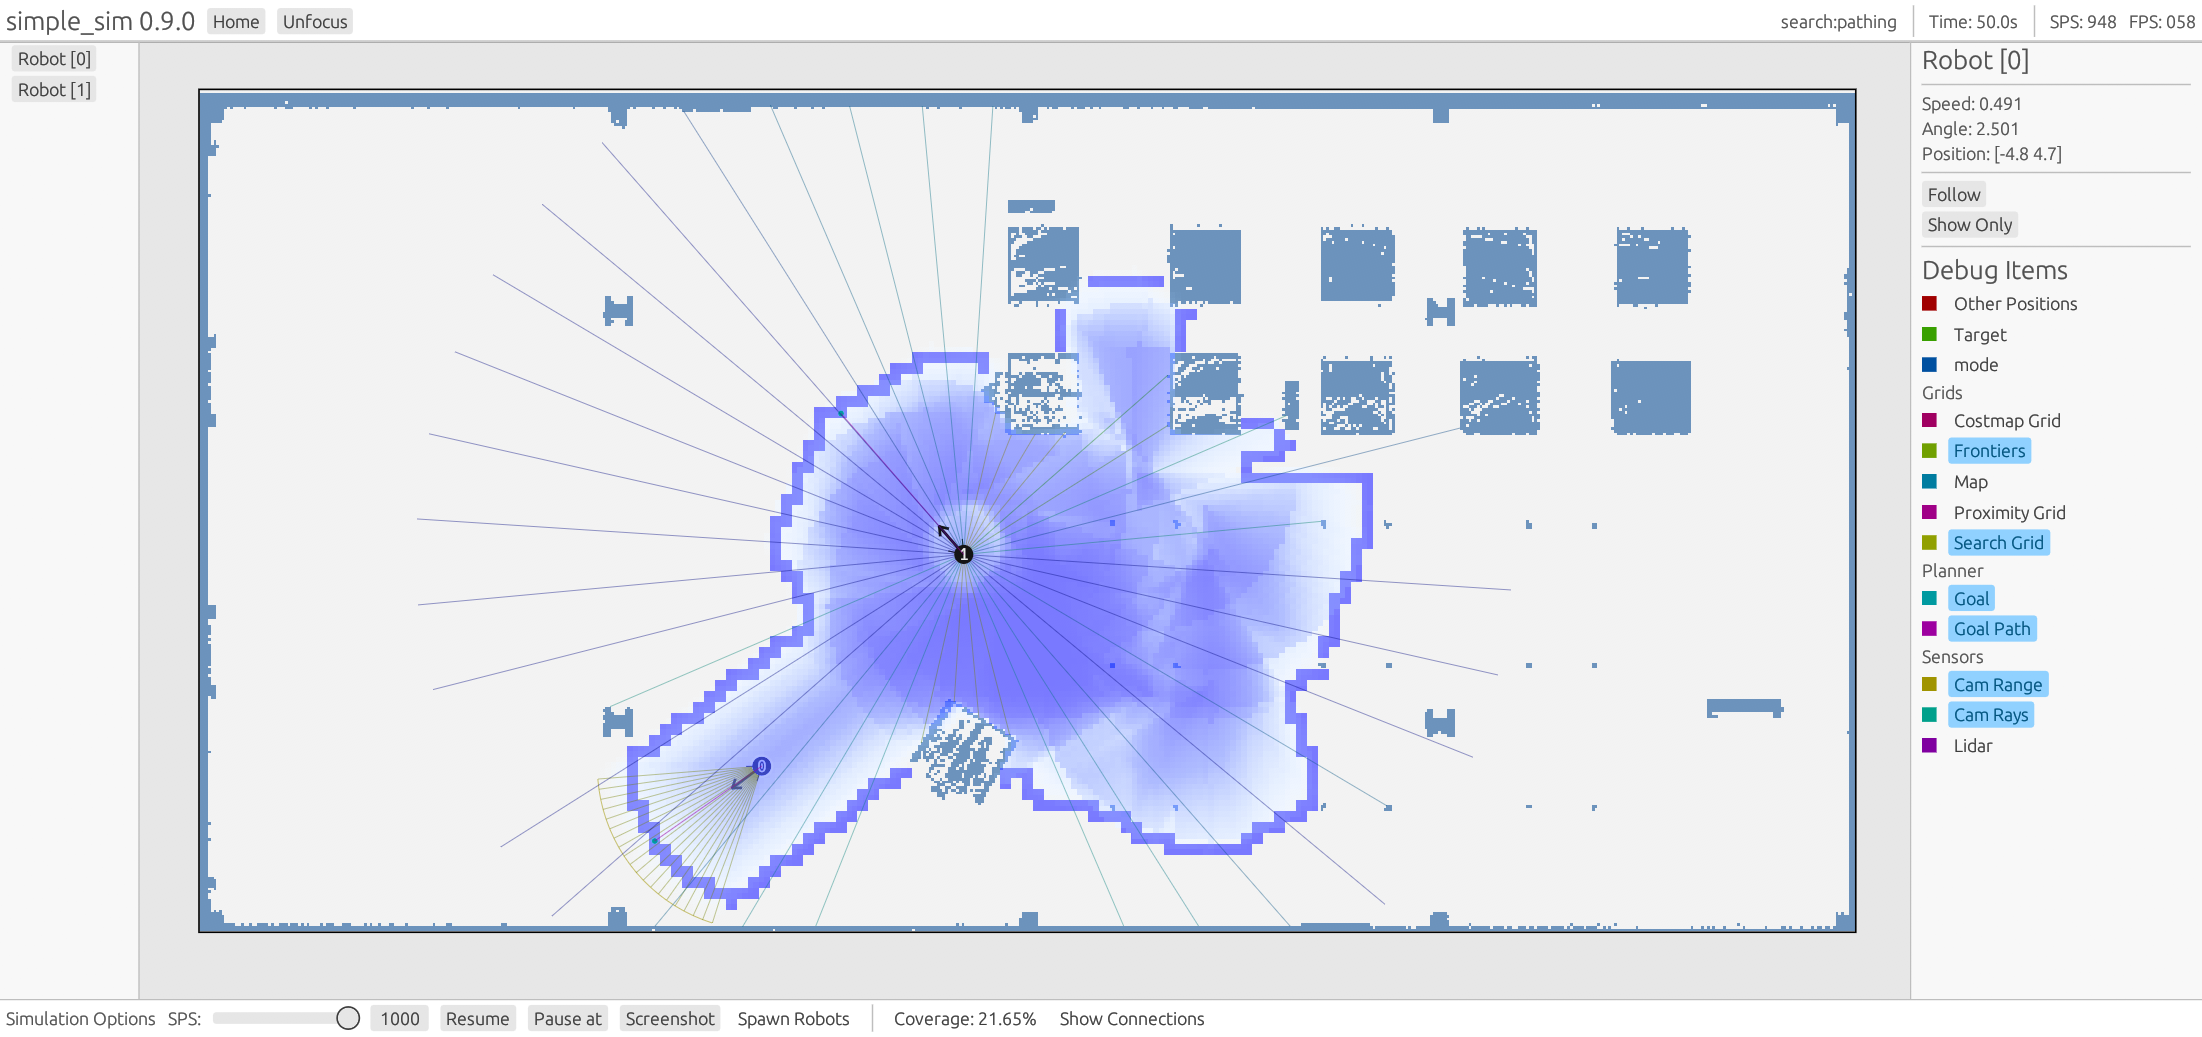
\includegraphics[width=\textwidth]{./figures/screenshots/simple_sim_depot.png}
        \caption{Simple Simulator Graphical User Interface showing two robots, one in the middle and one in the lower left part of the map. Several debug items are visualized: Search Grid, Frontiers, and LiDAR and Camera approximations are shown. These will be explained in later sections.}
        \label{fig:simple_sim}
    \end{subfigure} \\
    \vspace{3mm}
    \begin{subfigure}[b]{\w}
        \centering
        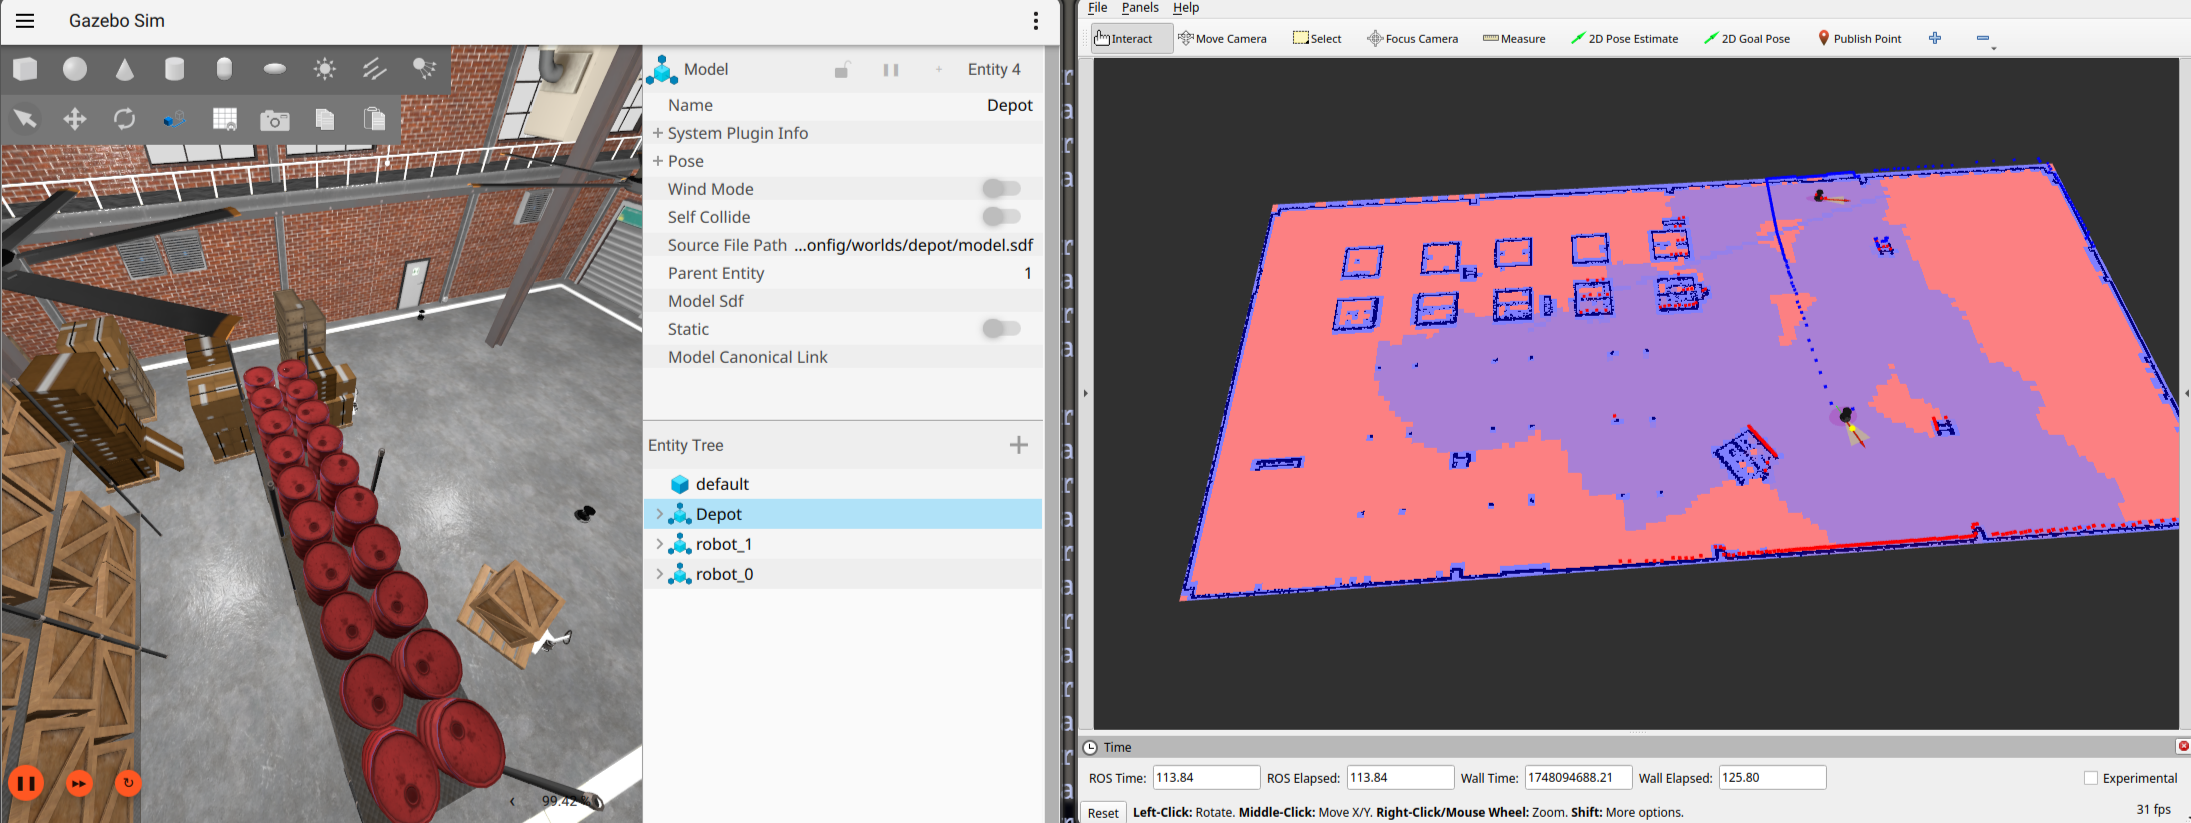
\includegraphics[width=\textwidth]{./figures/screenshots/gazebo_sim_depot.png}
        \caption{Gazebo Simulator in ROS 2. The left window contains the Gazebo visualization, which renders the 3D enviornment. On the right, RViz2 is visualizing data sent over topics which includes the current search grid as shown in red and blue.}
        \label{fig:gazebo_sim}
    \end{subfigure}
    \caption{Screenshots of the two simulators running the "depot" environment.}
    \label{fig:simulators}
\end{figure}

The double simulator architecture is built around the shared \texttt{botbrain} behavior library, which encapsulates each robot’s internal state and provides a standardized interface for behavior control. This modular design allows the same behavior code to be executed in both the lightweight \texttt{simple\_sim} environment and the more realistic Gazebo based simulation without requiring any code changes. By decoupling the behavior logic from the underlying simulation platform, the system supports consistent benchmarking and fair comparisons between algorithms. This separation also promotes cleaner, more testable, and reusable code, making it easier to iterate on behaviors and evaluate improvements.

\subsubsection{Behavior Debugging}
To facilitate development and validation, \texttt{botbrain} supports real-time debugging of both robot behavior and internal state, through the exposed debugging interface known as the \texttt{Debug Soup}. The \texttt{Debug Soup} allows behavior modules to annotate the simulation with structured debugging data. These debug items --- such as occupancy grids, path vectors, target points, and internal decision states --- can be visualized in both ROS 2 via RViz2 (\cref{fig:gazebo_sim}) and \texttt{simple\_sim} (\cref{fig:simple_sim}). \\

RViz2 supports visualization of messages published on ROS 2 topics. \texttt{Debug Soup} elements are converted into ROS 2 message formats (e.g. \texttt{OccupancyGrid}) and published for real-time display. In \texttt{simple\_sim}, debug items are located on the right panel in the user interface and their overlays can be toggled at will. \\

This enables introspection of robot behavior during simulations and is invaluable for development, debugging, and helps in interpreting emergent behavior of the swarm. The \texttt{Debug Soup} can be disabled to save memory and increase performance after development has finished.
